\section{example}
\begin{frame}{problem \cite{example}}
  \begin{figure}[htbq]
    \centering
    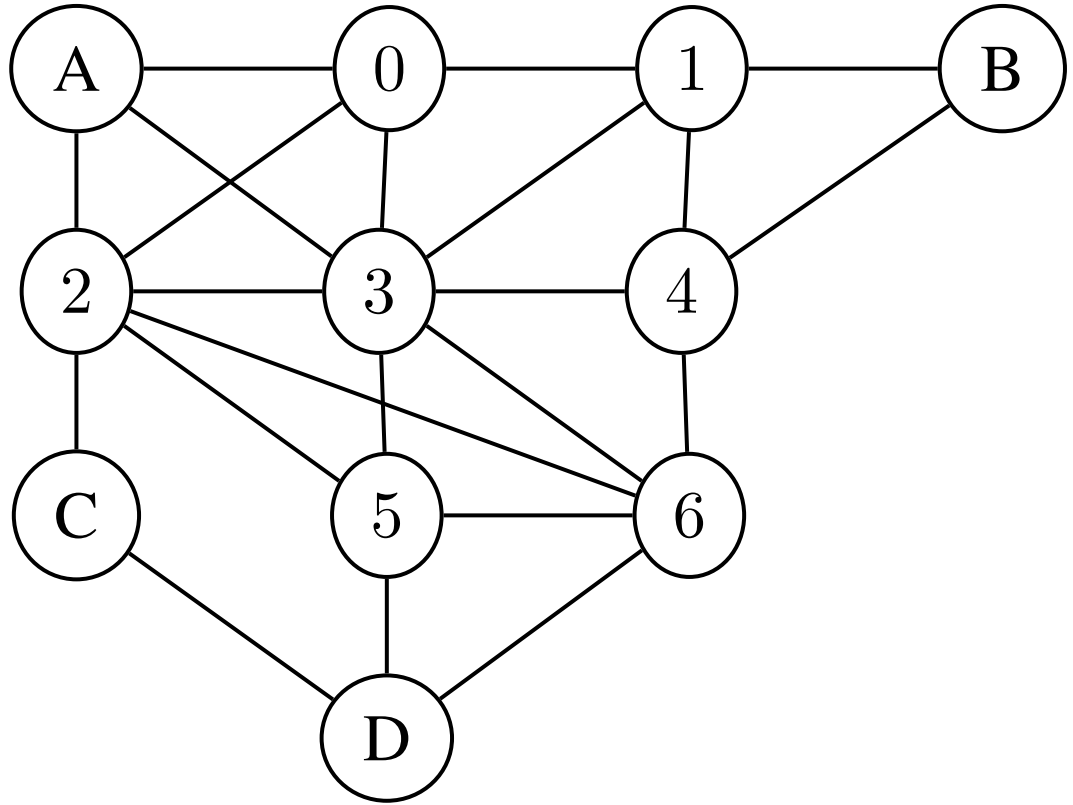
\includegraphics[width=0.5\textwidth]{figure/problem.png}
    \caption{Zed city as an undirected graph} 
    \label{fig-zed}
  \end{figure}
\end{frame}
\begin{frame}[fragile]
  \frametitle{boolean function}
  \begin{columns}
    \begin{column}{0.45\linewidth}
      \begin{block}{python implementation of f }
        \begin{lstlisting}[language=Python]
def f(v0, ..., v6 : BitVec(2)) -> BitVec(1):
  c0 = (v0 != ’00’)
  c1 = (v1 != ’01’) and (v1 != v0)
  c2 = (v2 != ’00’) and (v2 != ’10’) and (v2 != v0)
  c3 = (v3 != ’00’) and (v3 != v0) and (v3 != v1) and (v3 != v2)
  c4 = (v4 != ’01’) and (v4 != v1) and (v4 != v3)
  c5 = (v5 != ’11’) and (v5 != v2) and (v5 != v3)
  c6 = (v6 != ’11’) and (v6 != v2) and (v6 != v3) and (v6 != v4) and (v6 != v5)
  return c0 and c1 and c2 and c3 and c4 and c5 and c6
          \end{lstlisting}
      \end{block}
    \end{column}
    \begin{column}{0.45\linewidth}
      \begin{block}{hand-optimized python implementation of f }
        \begin{lstlisting}[language=Python]
def f(v0, ..., v6 : BitVec(2)) -> BitVec(1):
  c1 = (v1[0] == v1[1]) and (v3 != v1)
  c023 = ((v0 ˆ v2 ˆ v3) == ’00’)
  c4 = (v4 != v1) and (v4 != v3)
  c5 = (v5 != v2) and (v5 != v3)
  c6 = ((v2 ˆ v3 ˆ v5 ˆ v6) == ’00’) and (v6 != v4)
  return c1 and c023 and c4 and c5 and c6
          \end{lstlisting}
      \end{block}
    \end{column}
  \end{columns}
\end{frame}

\begin{frame}{flow}
  \begin{itemize}
    \item Angel:prepare a uniform quantum state
    given as input a Boolean function
    \item Tweedledum:synthesizing,
    manipulating, and optimizing quantum circuits
    \item Caterpillar:automatically translate the combinational parts of a quantum
    algorithm into quantum gates
  \end{itemize}
\end{frame}
\begin{frame}{initial state \footfullcite{initial}}
  \begin{itemize}
    \item target:
    \begin{align}
      \left|\varphi_{j}\right\rangle= \frac{1}{\sqrt{|on(f)|}} \sum_{x \in \operatorname{on}(f)}|x\rangle
    \end{align}
    \item the  general  idea  of  state  preparation  algorithm  relies on the identity:
    \begin{align}
      \mathrm{QSP}_{f}|0\rangle^{\otimes n} = \left(\mathrm{QSP}_{f_{\bar{x}_{i}}} \oplus \mathrm{QSP}_{f_{x_{i}}}\right)\left(G\left(p_{f}\left(\bar{x}_{i}\right)\right) \otimes I_{2^{n}-1}\right)|0\rangle
    \end{align}
    \item $G\left(p_{f}\left(\bar{x}_{i}\right)\right)$ is a unitary transformation gate that satisfies:
    \begin{align}
      G(p_{f}\left(\bar{x}_{i}\right))|0\rangle = \sqrt{p_{f}\left(\bar{x}_{i}\right)}|0\rangle+\sqrt{1-p_{f}\left(\bar{x}_{i}\right)}|1\rangle
    \end{align}
    \begin{align}
      G\left(p_{f}\left(\bar{x}_{i}\right)\right) = R_{y}\left(2 \cos ^{-1}\left(\sqrt{p_{f}\left(\bar{x}_{i}\right)}\right)\right)
    \end{align}
  \end{itemize}
\end{frame}
\begin{frame}
  \begin{figure}[htbq]
    \centering
    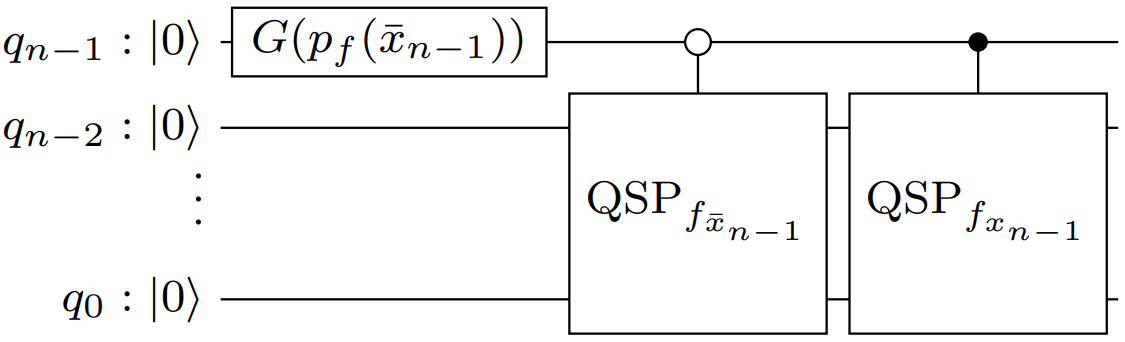
\includegraphics[width=0.9\textwidth]{figure/QSP.png}
    \caption{the general idea of QSP in the quantum  circuit  model for $i=n-1$.} 
    \label{fig-qsp}
  \end{figure}
\end{frame}
\begin{frame}{initial state example}
  \begin{figure}[htbq]
    \centering
    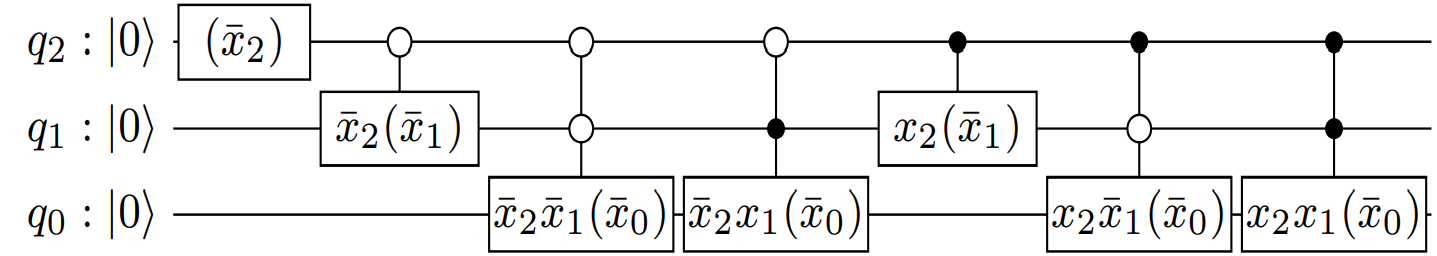
\includegraphics[width=0.9\textwidth]{figure/qsp_example.png}
    \caption{the abstract quantum gates of $QSP_{<x_0x_1x_2>}$} 
    \label{fig-qsp-example}
  \end{figure}
\end{frame}
\begin{frame}
  \begin{figure}[htbq]
    \centering
    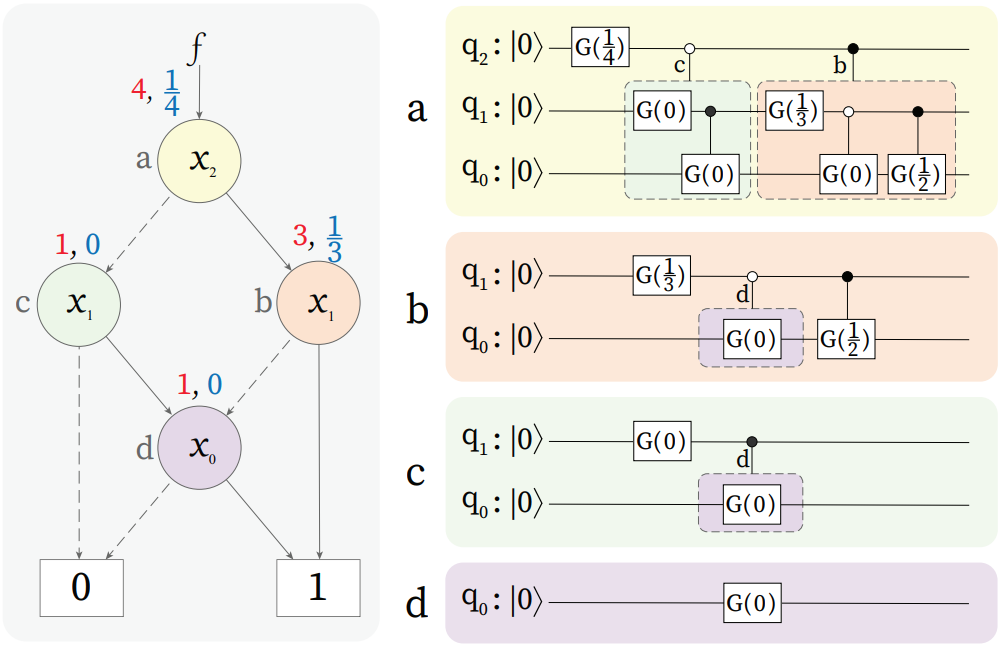
\includegraphics[width=0.8\textwidth]{figure/qsp_circuit.png}
    \caption{BDD  for boolean function $f= x_0x_1\vee x_1x_2 \vee x_2x_0 $ and  the  procedure  of  extracting  gates  for  each node from bottom to top} 
    \label{fig-qsp-example-circuit}
  \end{figure}
\end{frame}
\begin{frame}{compiling oracle by XAG\footfullcite{multiplicative}}
  \begin{itemize}
    \item representing an n-variable boolean function using a logic network over the gate basis$\{\lnot ,\oplus ,\wedge \}$:
    \begin{align}
      x_{i} = x_{j(i)} \oplus x_{k(i)} \quad \text { or } \quad x_{i} = x_{j(i)}^{p(i)} \wedge x_{k(i)}^{q(i)}
    \end{align}
    where $n\leq i < n+r$
    \item  the linear transitive fan-in of a node $x_i $using the recursive function:
    \begin{align}
      \operatorname{ltfi}\left(x_{i}\right) = \left\{\begin{array}{ll}
      \left\{x_{i}\right\} & \text { if } i < n \text { or } \circ_{i}  = \wedge, \\
      \operatorname{ltfi}\left(x_{j(i)}\right) \triangle \operatorname{ltfi}\left(x_{k(i)}\right) & \text { otherwise }
      \end{array}\right.
    \end{align}
  \end{itemize}
\end{frame}
\begin{frame}{XAG}
  \begin{algorithm}[H]
    \caption{compute} 
    \label{alg-be} 
    \begin{algorithmic}
      \REQUIRE Logic network with gates $x_n, \ddots, x_{n+r-1}$
      \ENSURE Quantum circuit for $Uf$

      \STATE set  $p \leftarrow p(i), q \leftarrow q(i), j \leftarrow j(i), k \leftarrow k(i) $
      \STATE set  $L_{1} \leftarrow \operatorname{ltfi}\left(x_{j}\right), L_{2} \leftarrow \operatorname{ltfi}\left(x_{k}\right) $
      \IF{$L_{1} \subseteq L_{2}$}
      \STATE swap $L_1 \leftrightarrow L_2$ and $p \leftrightarrow q$
      \ENDIF
      \STATElet  $t_{1}$  be some element in  $L_{1}\backslashL_{2}$
      \STATElet  $t_{2}$  be some element in  $L_{2}$
      \STATECNOT  $\left(x, t_{1}\right)$  for all  $x \in L_{1} \backslash\left\{t_{1}\right\}$
      \STATECNOT  $\left(x, t_{2}\right)$  for all  $x \in L_{2} \backslash\left\{t_{2}\right\}$
      \STATE if  p  then  $\operatorname{NOT}\left(t_{1}\right)$ 
      \STATE if  q  then  $\operatorname{NOT}\left(t_{2}\right)$ 
      \STATE$\operatorname{TOFFOLI}\left(t_{1}, t_{2}, x_{i}\right) $
    \end{algorithmic} 
  \end{algorithm}
\end{frame}
\begin{frame}{XAG example}
  \begin{itemize}
    \item for $f(x)=x_0x_1\vee x_1x_2\vee x_2x_0$
    \item we 
    \begin{align}
      x_{4} & = x_{1} \oplus x_{2}, & x_{5} & = x_{2} \oplus x_{3} \\
      x_{6} & = x_{4} \wedge x_{5}, & x_{7} & = x_{2} \oplus x_{6}
    \end{align}
  \end{itemize}
\end{frame}
\begin{frame}{XAG example}
  \begin{itemize}
    \item for $f(x)=x_0x_1\vee x_1x_2\vee x_2x_0$
    \item we 
    \begin{align}
      x_{4} & = x_{1} \oplus x_{2}, & x_{5} & = x_{2} \oplus x_{3} \\
      x_{6} & = x_{4} \wedge x_{5}, & x_{7} & = x_{2} \oplus x_{6}
    \end{align}
  \end{itemize}
\end{frame}
\begin{frame}{XAG example}
  \begin{figure}[htbq]
    \centering
    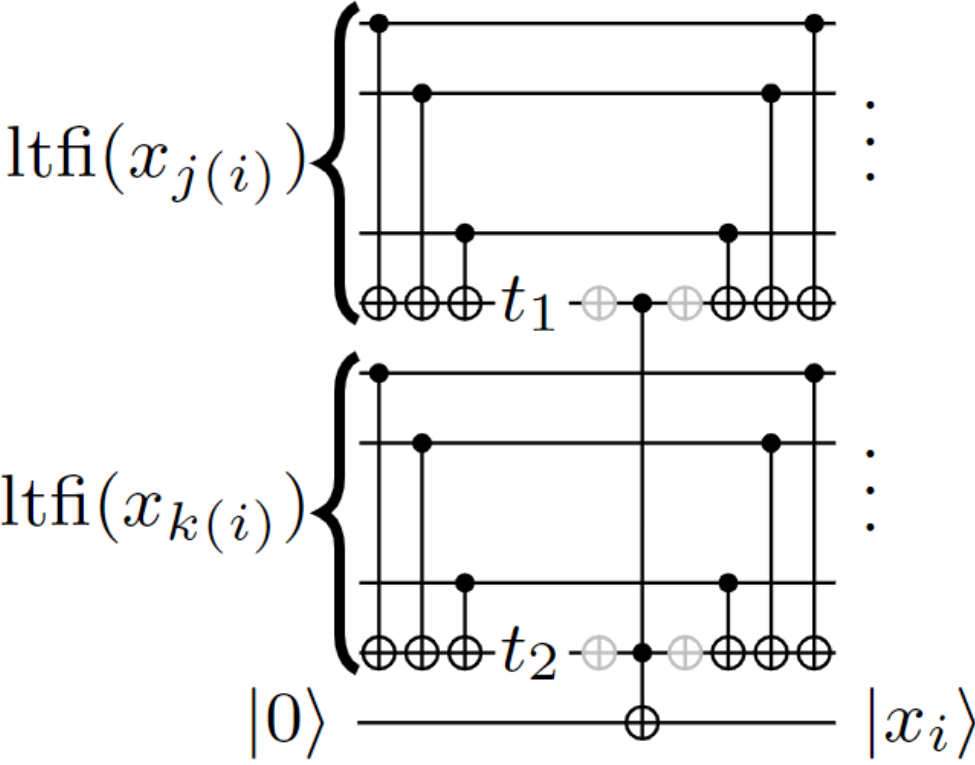
\includegraphics[width=0.5\textwidth]{figure/construction.png}
    \caption{Quantum circuit construction for AND step in XAG} 
    \label{fig-XAG}
  \end{figure}
\end{frame}
\begin{frame}{result}
  \begin{table}[htbq]
    \begin{tabular}{@{}lllll@{}}
    \toprule
    \multirow{2}{*}{} & \multicolumn{2}{c}{\text { Hand-optimized }} & \multicolumn{2}{c}{\text { Non-optimized }} \\ \cmidrule(l){2-5} 
                      &  \text { Qubits } & \text { cost } & \text { Qubits } & \text { cost } \\ \hline
    \text { IBM's solution } & 32 & 5004 & & \\
    \text { Whit3z solution } & 32 & 2474 & & \\
    \text { XAG-based flow } & 31 & 2202 & 56 & 4347 \\
    \text { XAG-based flow with pebbling } & 21 & 4497  & 30 & 7737 \\
    \bottomrule
    \end{tabular}
    \caption{quality  of results for boolean function (hand-optimized and non-optimized), where $cost = q_1+10q_2$}
  \end{table}  
\end{frame}
